% Document information
\newcommand{\titleinfo}{Zusammenfassung JavaC}
\newcommand{\authorinfo}{Sandro Pedrett}
\newcommand{\version}{1.0}
\newcommand{\versioninfo}{FS21}
% Header
\include{Template/Header}

% Setup Source Code
\lstset{ 
	backgroundcolor=\color{white},   % choose the background color; you must add \usepackage{color} or \usepackage{xcolor}; should come as last argument
	basicstyle=\footnotesize,        % the size of the fonts that are used for the code
	breakatwhitespace=true,         % sets if automatic breaks should only happen at whitespace
	breaklines=true,                 % sets automatic line breaking
	captionpos=b,                    % sets the caption-position to bottom
	commentstyle=\color{ForestGreen},    % comment style
	escapeinside={\%*}{*)},          % if you want to add LaTeX within your code
	extendedchars=true,              % lets you use non-ASCII characters; for 8-bits encodings only, does not work with UTF-8
	frame=single,	                   % adds a frame around the code
	keepspaces=true,                 % keeps spaces in text, useful for keeping indentation of code (possibly needs columns=flexible)
	language=Java,                      % the language of the code
	numbersep=5pt,                   % how far the line-numbers are from the code
	rulecolor=\color{black},         % if not set, the frame-color may be changed on line-breaks within not-black text (e.g. comments (green here))
	showspaces=false,                % show spaces everywhere adding particular underscores; it overrides 'showstringspaces'
	showstringspaces=false,          % underline spaces within strings only
	showtabs=false,                  % show tabs within strings adding particular underscores
	stepnumber=2,                    % the step between two line-numbers. If it's 1, each line will be numbered
	tabsize=2,	                   % sets default tabsize to 2 spaces
	title=\lstname,                   % show the filename of files included with \lstinputlisting; also try caption instead of title
	stringstyle=\ttfamily\color{red!50!brown},
	keywordstyle=\color{blue}\bfseries,
}

% 6 A4 Seiten

% Document
\begin{document}

\input{Sections/Einfürhung}
\section{Objekt Orientiertes Programmieren - OOP}
Wie jede OOP Sprache unterstützt auch Java das Konstrukt der Klassen, Vererbung und Polymorphismus. Eine \textbf{Klasse} ist eine Art Bauplan, hingegen ein \textbf{Objekt} die erstellten Gebäude ansich sind. Die \textbf{Instanz} ist ein einzigartiges Objekt, in diesem Fall ein spezifisches Gebäude. Instanzen werden mit dem Operator \textit{new} erstellt.
\begin{lstlisting}
	Buildung b = new Buildung();
\end{lstlisting}
Wichtig ist, dass jedes Objekt in Java vom Basisobjekt \textit{Object} erbt. Desshalb sind auf allen Instanzen folgende Methoden verfügbar:
\begin{itemize}[nosep]
	\item public String toString()
	\item public boolean equals(Object obj)
	\item public int hashCode()
\end{itemize}

\subsection{Methoden}
Methoden können in Klassen definiert werden. Diese Methode ist jedoch an das Objekt gebunden und kann Instanzvariablen modifizieren. Ausser Methode oder Instanzevariable ist mit \textit{static} deklariert.

Duch Generics (1) können auch einzelne Methoden verallgemeinert werden. Falls eine offene Anzahl an Parametern benötigt wird, können Varargs (2) eingesetzt werden.
\begin{lstlisting}
// (1)
public <E> Stack<E> getStack(E value, int times) { }
public <E> void push(E... items) { }
\end{lstlisting}


\subsection{Vererbung}
Java unterstützt die Vererbung mittels den Keywords \textit{extends} und \textit{implements} für Interfaces.\\
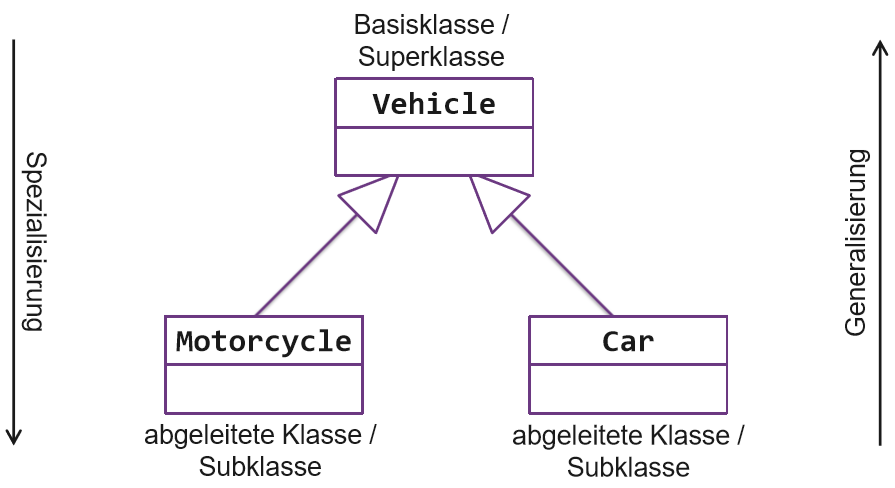
\includegraphics[width=\columnwidth]{Images/vererbung}

Die Vererbung kann durch Generics eingeschränkt werden
\begin{lstlisting}
class GraphicStack<T extends Graphic> extends Stack<T> {
	...
}
\end{lstlisting}


\subsection{Overloading}
Das Konzept von overloading beschreibt die Möglichkeit Methoden zur Laufzeit (dynamisch) zu überschreiben. Wenn abstract verwendet wird, kann der Kompiler die Methode bereits statisch evaluieren.

\begin{lstlisting}
	public class Programm {
		public static void main(String args[]) {
			Car c = new Car();
			Vehicle v =  c;
			v.print();	// prints: Car
			c.print();  // prints: Car
			
			v = new Vehicle();
			v.print();	// prints: Vehicle
		}
	}
	
	class Vehicle {
		public String getKind () {
			return "Vehicle";
		}
		
		public void print() {
			System.out.println(getKind());
		}
	}
	
	class Car extends Vehicle {
		@Override
		public String getKind() {
			return "Car";
		}	
	}
\end{lstlisting}

\textbf{Wichtig:} Attribut \textit{@Override} ist freiwillig, der Kompiler weist jedoch bei Fehlender Basis Method auf einen Fehler hin.
\section{Collections}
Java unterstützt bereits viele verschiedene Collections. Eine Collection ist eine Ansammlung von Daten. Die wichtigsten sind:\\
\begin{tabular}{lll}
	Interface & Beschreibung & Beispiel Implementation \\ \toprule
	List & Folge von Elementen & $ArrayList<T>$ \\
	Set & Menge von Elementen & $HashSet<T>$ \\
	Map & Key-Value Pair & $HashMap<K, V>$ \\
\end{tabular}
\section{Exceptions}
Exceptions sind Ausnahmefälle welche durch den \textit{try-catch}-Block abgefangen werden können. Es gibt in Java zwei unterschiedliche Arten von Exceptions: 
\begin{itemize}[nosep]
	\item Error
	\item Exception
\end{itemize}

\noindent Dabei sind \textbf{Error} schwerwiegende Fehler die \underline{nicht behandlet} werden sollen zB OutOfMemoryError, StackOverflowError etc. Hingegen sind \textbf{Exception} Laufzeitfehler die \underline{behandelbar} sind zB IOException.


\subsection{Unchecked vs Checked}
In Java müssen alle Exceptions welche eine checked Objekt werfen, diese in der Deklaration beinhalten bzw werden vom Kompiler geprüft. Unchecked Exceptions sind RuntimeExceptions sowie Error und deren Unterklassen welche nicht vom Kompiler geprüft werden. 
\begin{lstlisting}
static String readFile(String path) throws IOException {
	if (path == null) throw new NullPointerException("No Path");
	
	throw new IOException("Not implemented yet");
}

void testMethod() {
	try {
		readString("test.txt");
	} catch (IOException | NullPointerException e) {
		e.printStackTrace();
	} finally {
		System.out.println("Finished");
	}
}
\end{lstlisting}
\begin{center}
	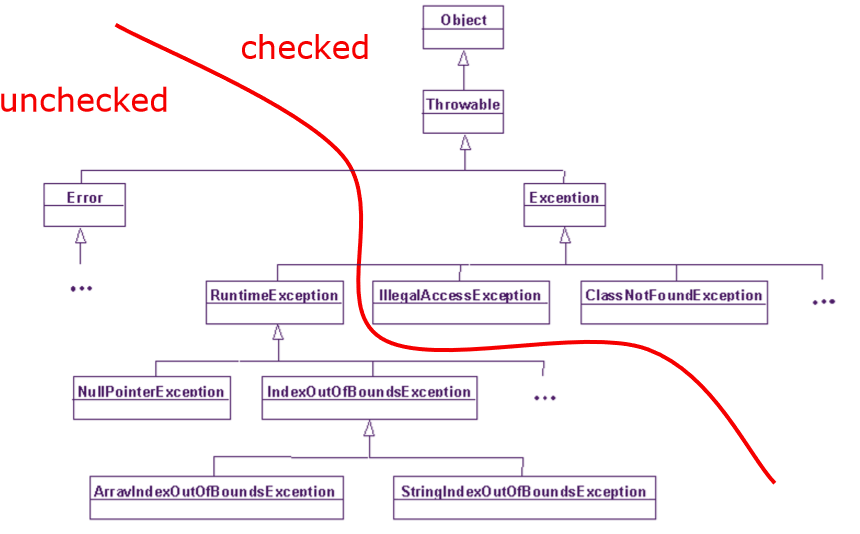
\includegraphics[width= 0.8\columnwidth]{Images/exception_uc}
\end{center}

\subsection{Resources}
Wenn eine Klasse \textit{AutoClosable} implementiert, kann sie automatisch geschlossen werden mit einem Try-With-Resources block
\begin{lstlisting}
try (Scanner s = new Scanner(System.in)) {
	// work with s
}
\end{lstlisting}
\section{Stream API}
\subsection{Lambda}
Lambda Ausdrücke sind quasi Methoden ohne Namen und können in Streams oder als Parameter übergeben werden, um verschiedene Vergleiche auszuwerten.


Lambdas können Ad-Hoc erzeugt werden, dabei muss die Signature aka Paramter und Rückgabewert übereinstimmen.
\begin{lstlisting}
people.sort((Person p1, Person p2) -> {
	return Integer.compare(p1.getAge(), p2.getAge());	
});
\end{lstlisting}

\textit{@FunctionalInterface} beschreibt dem Kompiler, das in diesem Interface nur eine Methode stehen darf.
\begin{lstlisting}
@FunctionalInterface
interface Comperator<T> {
	int compare(T first, T second);
}


class Person {
	int compareByAge(Person p1, Person p2) {
		return Integer.compare(p1.getAge(), p2.getAge());	
	}
}

Comperator<Person> myComparison = this::compareByAge;
\end{lstlisting}

\subsection{Stream}
Eine anwendung von Lambdas sind Stream API notationen. Dabei sollen zB Listen durch Filtern und/oder Sortieren modifiziert werden. Dafür muss eine \textit{Stream} erzeugt werden auf welchen Operationen parallel oder seqentiell ausgeführt werden können. Der Verarbeitungskette seht immer ähnlich aus

\begin{center}
	\begin{minipage}{0.2\textwidth}
		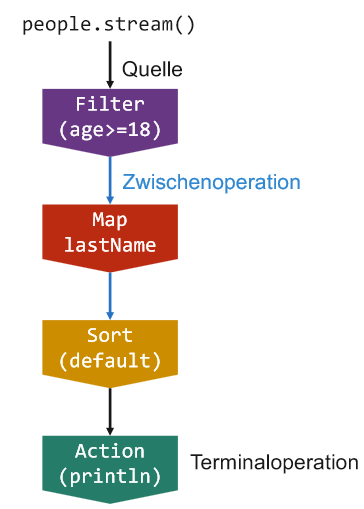
\includegraphics[width=\columnwidth,keepaspectratio=true]{Images/stream}
	\end{minipage}%%% to prevent a space
	\begin{minipage}{0.3\textwidth}
		\begin{lstlisting}
poeple.stream()
	.filter(p -> p.getAge() >= 18)
	.map(p -> p.getLastName())
	.sorted()
	.forEach(System.out::println);
		\end{lstlisting}
	\end{minipage}
\end{center}

\noindent\textbf{Wichtig:} Keine Interfernz, Collection darf \underline{nicht} verändert werden (1) oder Abhängikeiten zu äusseren, änderbaren Variablen haben (2) .
\begin{lstlisting}
// (1)
filter(p -> people.add(p))	
			
// (2)			
map(p -> {globalCounter++; return p;})	
\end{lstlisting}

\subsection{Operationen}
\begin{tabular}{p{4cm}p{5cm}}
	filter(Predicate) & Filtern mit Predicate-Funktionsobjekt/Lamda \\ \midrule
	map(Function) & Proijziert auf Rückgabewert von Funktionsobjekt/Lambda \\ \midrule
	mapToInt/Long/Double & Proijziert auf int,long,double \\ \midrule
	sorted() & Sortiert mit/Ohne Comperator \\ \midrule
	distinct() & Duplikate entfernen (equals()) \\ \midrule
	limit(long n) & Bis Element n liefern \\ \midrule
	skip(long n) & AB Element n liefern 
\end{tabular}
\section{IO}
Grundsätzlich werden IO-Streams mit Byte Stream \textit{InputStram, OutputStream} mit zB \textit{FileInputStream, FileOutputStream} erzeugt. Für UTF-16 können konkret die \textit{Reader, Writer} für Zeichen-/Zeilenweise Ein-\& Ausgabe verwerndet werden.

\noindent Java bietet auch direkten Daten-Zugriff durch die statische Klasse Files an. \textbf{Achtung:} Benötigen IOException!
\begin{itemize}[nosep]
	\item Files.readAllBytes(Path.of(str))
	\item Files.write(Path.of(str), data)
	\item Files.readAllLines(Path.of(str), StandardCharsets.UTF\_8) : List[String]
	\item Files.lines(Path.of(str), StandardCharsets.UTF\_8) : Stream[String]
	\item Files.write(Path.of(str), lines, StandardCharsets.UTF\_8)
\end{itemize}

\subsection{Stream}
Jeder Stream muss wieder geschlossen werden, ansonsten muss mit Datenverlust gerechnet werden.
\begin{lstlisting}
try (var in = new FileInputStream(path)) {
	int c = in.read();
	while (c >= 0) {
		byte b  = (byte)c;
		
		c = in.read();
	}
}
\end{lstlisting}

\subsubsection{Standard Input/Output}
Folgende Standard Streams werden verwendet um standardmässig auf die Konsole zu Schreiben.
\begin{itemize}[nosep]
	\item System.in
	\item System.out
	\item System.err
\end{itemize}

\subsection{Reader/Writer}
In Java ist der char-Type ein 16Bit (UTF-16) kodierung. Hier einige Beispiele:
\begin{lstlisting}
	try (var in = new FileReader(path)) {
		int c = in.read();
		while (c >= 0) {
			char b  = (char)c;
			
			c = in.read();
		}
	}
\end{lstlisting}

\begin{lstlisting}
	try (var writer = new FileWriter(path, append)) {
		writer.write("Hallo!");
		wirter.write('\n');
	}
\end{lstlisting}

\noindent Für \textbf{Buffered}Reader-/ Writer ist es wichtig, \textit{flush()} aufzurufen. Dies erzwingt den Reader/-Writer alle gepufferten Werte sofort zu Schreiben bzw. Lesen. \textit{close()} ruft impliziet \textit{flush()} auf. Dies wird für Performance-Gründen eingesetzt.

\section{GUI}
Swing ist ein altes Java-Framework um GUI (Graphical User Interface) zu erstellen (Neuer wäre zB JavaFX). GUIs sind dazu da, um Informationen mit dem Benutzer auszutauschen und ein spezifisches Layout (Anordnung der Elemente etc) festzulegen. Damit werden Interkation zwischen Program und Benutzer möglich. Auch eine Consolen-Anwendung ist ein sehr einfach gehaltenes GUI.

\begin{center}
	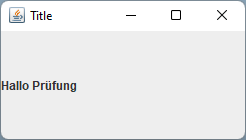
\includegraphics[width=0.3\columnwidth]{Images/swing1}
\end{center}
\begin{lstlisting}
import javax.swing.*;
	
public class HelloSwing {
	public static void main(String[] args) {
		JFrame frame = new JFrame("Title");
		frame.setSize(100, 30);
		
		frame.setDefaultCloseOperation(JFrame.EXIT_ON_CLOSE);
		
		JLabel label = new JLabel("Hallo Pruefung");
		frame.getContentPane().add(label);
		frame.pack(); // Minimal Groesse einnehmen
		frame.setVisible(true);
	}
}
\end{lstlisting}




\subsection{Event-Dispatch-Thread}
Jede Java Swing Applikation besitzt ein eigenen Event-Loop (Event-Dispatch-Thread EDT) welcher Events vom Native-Event-Loop an die Zuständige Komponente weiterleitet. Der Native-Event-Loop ist eine Zwischenstuffe um die Platform unabhängigkeit zum jeweliigen OS zu gewährlsiten. Events sind Ereignisse zB Tastendruck oder Mausklick, welche zum jeweiligen Program bzw. der entsprechenden Komponente weitergeleitet werden müssen. Mittels \textit{ActionListener} Interface können diese in der Komponenten registiert werden.

ActionListener werden häufig mit Lambdas oder Inner-Klassen implementiert.
\begin{lstlisting}
button1.addActionListener((e) -> {
		JFileChooser fc = new JFileChooser();
		fc.showOpenDialog(null);
	}
});

button1.addActionListener((e) -> {
		System.exit(0);
	}
});
\end{lstlisting}


\subsection{Layout-Manager}
\begin{tabular}{m{1cm} m{100px} m{4cm}}
	\textbf{Name} & \textbf{Beispiel} & \textbf{Eigenschaften} \\ \toprule
	Border & 	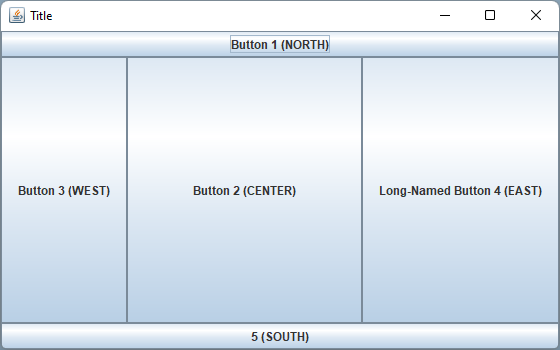
\includegraphics[width=100px]{Images/borderlayout} & \begin{itemize}[nosep]
		\item CENTER-Fläche wird maximiert
		\item Reihenfolge von add() irrelevant
		\item One Positionsangabe bei add(): CENTER
	\end{itemize} \\ \midrule
	Box & 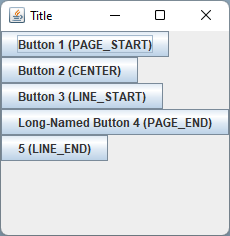
\includegraphics[width=100px]{Images/boxlayout} & \begin{itemize}[nosep]
		\item Komponenten werden in einer Reihe oder Spalte ausgegeben
		\item Alignment supported
		\item Vordert Maximale Grössen
	\end{itemize}  \\\midrule
	Card & 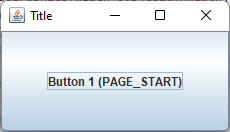
\includegraphics[width=100px]{Images/cardlayout} & \begin{itemize}[nosep]
		\item Überlagert Komponenten zB für TabbedPane oder JComboBox
	\end{itemize} \\\midrule
	Flow & 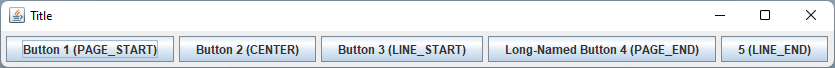
\includegraphics[width=100px]{Images/flowlayout} & \begin{itemize}[nosep]
		\item Komponenten werden in einer Riehe oder Spalte ausgegeben sofern Platz vorhanden
		\item Standard von JPanel
	\end{itemize} \\\midrule
	GridBag & 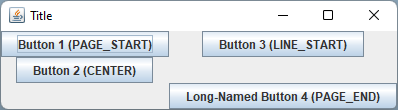
\includegraphics[width=100px]{Images/girdbag} & \begin{itemize}[nosep]
		\item Komponenten können mehrer Zellen besitzen
		\item Unterschiedliche Höhen und Breiten von Zellen
	\end{itemize} \\\midrule
	Grid & 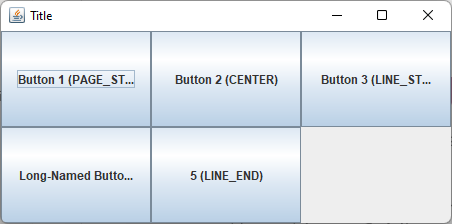
\includegraphics[width=100px]{Images/gridlayout} & \begin{itemize}[nosep]
		\item Macht Anzahl von Spalten und Zeilen gemäss Konstruktur
		\item Reihenfolge von add() bestimmt Anordnung
		\item Alle Zellen gleich gross
	\end{itemize} \\\midrule
		
\end{tabular}
	
\textbf{Beispiel}
\begin{lstlisting}
import javax.swing.*;
import java.awt.*;

public class MainProgram {
	public static void main(String[] args) {
		JFrame frame = new JFrame("Title");
		frame.setLayout(new BorderLayout());
		
		Container panel = frame.getContentPane();
		
		JButton button = new JButton("Button 1 (NORTH)");
		panel.add(button, BorderLayout.NORTH);
		
		button = new JButton("Button 2 (CENTER)");
		panel.add(button, FlowLayout.CENTER);
		
		button = new JButton("Button 3 (WEST)");
		panel.add(button, BorderLayout.WEST);
		
		button = new JButton("Long-Named Button 4 (EAST)");
		panel.add(button, BorderLayout.EAST);
		
		button = new JButton("5 (SOUTH)");
		panel.add(button, BorderLayout.SOUTH);
			
		frame.pack();
		frame.setVisible(true);
	}
}
\end{lstlisting}

	
\subsection{Swing Komponenten}
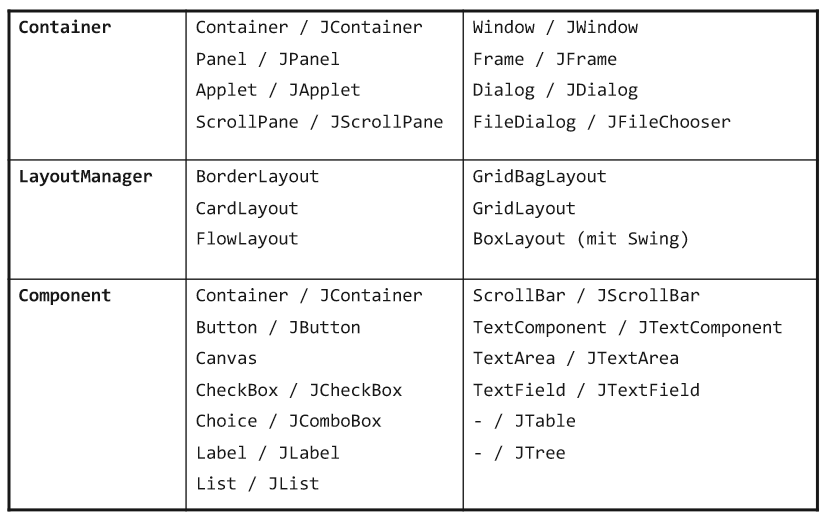
\includegraphics[width=\columnwidth]{Images/swing_komponenten}

	

\section{Testen}
Ofte werden für UnitTests Äuivalenzklassen gebildet welche Parameter in Bereich zerlegen, die von der Funktion wahrscheinlich gleich behandelt werden. Für jeden Bereich eine Eingangsvariable wählen und Testfall schreiben.

\subsection{JUnit Framework}
Die Testmethoden in JUnit haben keine Parameter und immer den Rückgabetype void. Sie sind mit der Annotation \textit{org.junit.jupiter.api.\textbf{@Test}} deklariert.

\begin{lstlisting}
@Test
void testMethod() {
	int negativeValue = -1;
	assertEquals(1, abs(negativeValue));	
}
\end{lstlisting}

Wichtige Asserts:
\begin{itemize}[nosep]
	\item assertEquals(expected, actual)
	\item assertEquals(expected, actual, delta)
	\item assertArrayEquals(expected, actual)
	\item assertTrue(actual)
\end{itemize}

\tableofcontents

\end{document}